\documentclass[twoside,a4paper,12pt]{report} %,draft,openright

\usepackage{polski}
\usepackage[utf8]{inputenc} 
\usepackage{gensymb}
\usepackage{epsf,graphicx}
\usepackage{subfigure}
\usepackage{latexsym,amssymb}
\usepackage{setspace,cite}
\usepackage{indentfirst}
\usepackage{mathtools}
\usepackage[justification=centering]{caption}
\usepackage{multirow}
\usepackage[figuresright]{rotating}

% for margins left, right top bottom
\usepackage{anysize}
\marginsize{3cm}{2.5cm}{2.5cm}{2.5cm}
\let\origdoublepage\cleardoublepage    %%komenda wstawiająca czyste kartki
\newcommand{\clearemptydoublepage}{%
  \clearpage
  {\pagestyle{empty}\origdoublepage}%
}
\let\cleardoublepage\clearemptydoublepage
\graphicspath{ {Resources/} }


%\usepackage{draft} %draft option - doesn't put full figures in -
            % useful when editing

%does the headers on the pages - keep in
\usepackage{fancyhdr}

%omitting any of these makes the thesis compile without the omitted
%chapter - good for editing single chapters.
%\includeonly{header,appendix}


\begin{document}
\newpage

%Puts page numbering of preamble in roman and of main body of thesis in
%arabic. Also defines how chapters and sections are made
\pagenumbering{arabic}
\setcounter{page}{1} \pagestyle{fancy}
\renewcommand{\chaptermark}[1]{\markboth{\chaptername%
\ \thechapter:\,\ #1}{}}
\renewcommand{\sectionmark}[1]{\markright{\thesection\,\ #1}}

%DEFINES TITLE PAGE, and contains abstract, acknowledgements, etc.

%%%%%%%%%%%%%%%%%%%%%%%%%%%%%%%%%%%%%%%%%%%%%%%%%%%%%%%%%%%%%%%%%%%%%%%%%%%
% This is a sample header for a sample dissertation. Fill in the name,
% and the other information. LaTeX will work out the table of
% content, the list of figures and of tables for you.
%%%%%%%%%%%%%%%%%%%%%%%%%%%%%%%%%%%%%%%%%%%%%%%%%%%%%%%%%%%%%%%%%%%%%%%%%%%

\newpage
\thispagestyle{empty}




% ******* Title page *******
% **************************

\begin{onehalfspacing}
\begin{center}

\centering

\includegraphics[keepaspectratio,scale=0.1]{./figures/godlo.PNG} \\[.8cm]


{\fontsize{17}{17}\selectfont
\textsc{Politechnika Śląska \\[.3cm]
Wydział Automatyki, Elektroniki i Informatyki  \\[.3cm]
Kierunek Informatyka  \\[2.5cm]}
\textbf{Praca dyplomowa magisterska \\[1.7cm]}}



\large 
{Algorytm wyszukiwania z tabu do rozwiązywania problemu układania planu zajęć} \\[3.1cm]
% Jeśli tytuł pracy zajmuje 2 linijki, wartość [2.3cm] zamieniamy na [3.1cm], jeśli tylko jedną - na [3.9cm] i odwrotnie - zwiększając liczbę linijek o jedną (do czterech) zmieniamy na [1.5cm] itd.


\large
\begin{flushleft}
Autor: Michał Szluzy  \\
Kierujący pracą:  prof. dr hab. inż. Zbigniew Czech \\
\end{flushleft}

\vspace{2cm}
Gliwice, czerwiec 2017
\end{center}
\end{onehalfspacing}

\singlespacing
\newpage

\thispagestyle{empty}
\mbox{}


%ABSTRACT
\begin{abstract}
W niniejszej pracy został opisany proces przystosowania algorytmu wyszukiwania z tabu do rozwiązywania problemu układania planu zajęć. Aspektem badawczym pracy było zbadanie wpływu parametrów zaimplementowanego algorytmu na szybkość jego działania i otrzymane wyniki. Omówione zostały podstawy teoretyczne badanego problemu oraz trudności towarzyszące implementacji algorytmu jego rozwiązania. Testowanie algorytmu zostało przeprowadzone na danych rzeczywistych, a wyniki zaprezentowane na wykresach.
\end{abstract}
%END OF ABSTRACT

\setcounter{page}{4} 
\doublespacing
\mbox{}

%\pagestyle{empty}
%\pagenumbering{Roman}
%\setcounter{page}{0} \pagestyle{plain}


\tableofcontents

\listoffigures
%\listoftables

\newpage
\thispagestyle{empty}


%\pagestyle{fancy}


\newpage

%sets up headers for lefthand and righthand pages. To alter, edit
%these lines and the chaptermark/sectionmark lines above
%\addtolength{\headheight}{3pt} \fancyhead{}
%\fancyhead[LE]{\sl\leftmark} \fancyhead[LO,RE]{\rm\thepage}
%\fancyhead[RO]{\sl\rightmark} \fancyfoot[C,L,E]{}
\pagenumbering{arabic}
\fancyhead[LE,RO]{\slshape \rightmark}
\fancyhead[LO,RE]{\slshape \leftmark}
\fancyfoot[C]{\thepage}


\setlength{\parskip}{1ex} %odstępy między akapitami
%\singlespacing
%\doublespacing
\onehalfspacing
\chapter{Wstęp}


Problem układania planu zajęć jest dobrze znany w środowiskach szkolnych i akademickich. Układanie planu to zajęcie żmudne oraz wymagające dużej spostrzegawczości i wyobraźni u osoby, która plan układa. Problem ten jest aktualny każdego roku, lub w przypadkach koniecznych np. przy zmianie liczby prowadzących, bądź zmienionej siatce zajęć. Układanie planu zajęć metodami tradycyjnymi pochłania dużo czasu i często kończy się niepowodzeniem. Jeżeli już uda się ułożyć plan, to często nie jest on najlepszy i nie spełnia oczekiwań uczniów bądź nauczycieli. Dlatego też badacze w wielu środowiskach na świecie rozważają problem układania planu zajęć i poszukują efektywnych algorytmów jego rozwiązania. W obecnych czasach mało która szkoła lub uczelnia nie wspomaga się przy tej czynności komputerem. Możliwość szybkiego utworzenia i ocenienia wielu planów lub uzyskanie wiedzy, czy dany plan jest możliwy do zrealizowania, to tylko niektóre zalety zastosowania do tego celu komputera. Najważniejszą zaletą jest możliwość skorzystania z algorytmów, które w krótkim czasie, np. 10 minut, ułożą plan zajęć zgodnie z podanymi założeniami.

Celem niniejszej pracy jest zbadanie możliwości zastosowania algorytmu wyszukiwania z tabu do problemu układania planu zajęć. Algorytm ten, rozwiązujący trudne problemy z wielu dziedzin życia, może być również zastosowany do rozwiązywania problemu układania planu zajęć. Praca oparta jest na materiałach źródłowych, w których do optymalizacji układania planu zajęć wykorzystano różne algorytmy heurystyczne. Korzystając z doświadczeń poprzedników, udało się uniknąć typowych błędów pojawiających się przy implementacji algorytmów rozwiązywania rozważanego problemu.

Aspektem badawczym pracy jest zbadanie wpływu parametrów zaimplementowanego algorytmu na szybkość jego działania i otrzymywane wyniki. Korzystając z dużej bazy danych testowych pochodzących z różnych szkół i uczelni na świecie dokonamy testowania algorytmu dla rzeczywistych problemów układania planu zajęć.

Praca, poza wstępem i zakończeniem, składa się z pięciu rozdziałów oraz jednego dodatku. Pierwszy rozdział poświęcony jest omówieniu algorytmu wyszukiwania z tabu. Przedstawiono w nim cechy algorytmów heurystycznych i metaheurystycznych oraz genezę algorytmu wyszukiwania z tabu. W rozdziale znaleźć można również omówienie podstawowej idei działania algorytmu oraz różnych jego wariantów. Zdefiniowano także podstawowe pojęcia związane z algorytmem, takie jak sąsiedztwo, kryterium aspiracji, dywersyfikacja, intensyfikacja, etc. Drugi rozdział formułuje problem układania planu zajęć. Zawiera formalizację problemu i omówienie ograniczeń związanych z planami zajęć. Przedstawiona jest również złożoność problemu układania planu zajęć w celu uzasadnienia potrzeby zastosowania algorytmów heurystycznych. Kolejny rozdział w całości poświęcony jest formatowi danych wejściowych, jakie są niezbędne do zaimplementowania algorytmu w celu poprawnego działania. Używany format danych jest wykorzystywany w problemie układania planu zajęć przez wielu badaczy na całym świecie. Opisanie formatu pozwala zrozumieć problemy, z jakimi trzeba się zmierzyć podczas implementowania algorytmu. Implementacja algorytmu oraz jego specyfikacja wewnętrzna i zewnętrzna zostały opisane w następnym rozdziale. Przedstawiono w nim funkcje wykorzystane w jej realizacji. Omówiono również wykorzystane podczas pracy narzędzia i środowiska. W ramach specyfikacji zewnętrznej przedstawiono opis interfejsu graficznego użytkownika oraz sposób korzystania z aplikacji. Ostatni rozdział opisuje proces testowania algorytmu. Omówiona została w nim specyfikacja środowiska testowego oraz zestaw danych wybrany do testowania. Wyniki działania aplikacji zostały zaprezentowane w postaci dwóch wygenerowanych planów zajęć wraz z oceną uzyskanych rozwiązań. Na końcu rozdziału zaprezentowano wpływ parametru długości listy tabu na wyniki działania algorytmu. Do pracy dołączono dodatek, w którym przedstawiono wybrane fragmenty kodu źródłowego.
\chapter{Problem układania planu zajęć}
\section{Sformułowanie problemu}
Problem układania planu zajęć można sformułować następująco. Dana jest lista określonych wydarzeń, dostepnych okien czasowych i zasobów. Należy przyporządkować wydarzeniom okna czasowe oraz zasoby w taki sposób, by spełnić przyjęte założenia (rysunek 3.1). W formułowanym problemie:
\begin{itemize}
	\item wydarzeniami są poszczególne lekcje odbywające się w ciągu jednego tygodnia,
	\item dostępnymi oknami czasowymi są godziny w których mogą odbywać się zajęcia (np. od poniedziałku do piątku w godzinach między 8:00 a 18:00),
	\item zasoby to dostępne sale lekcyjne, nauczyciele prowadzący zajęcia, grupy uczniów itp.
\end{itemize}


\begin{figure}
	\centering
	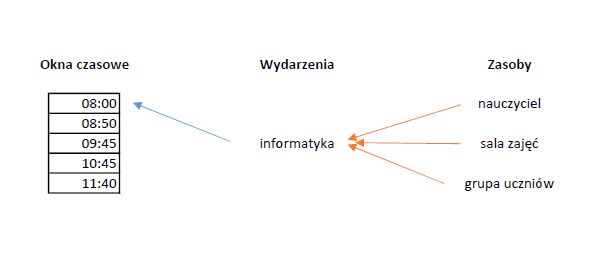
\includegraphics{podzialzasobow}
	\caption{Ilustracja problemu układania planu zajęć}
	\label{fig: podzialzasobow}
\end{figure}

Układanie planu zajęć wymaga spełnienia określonych ograniczeń. Mianowicie nie można wypełnić dostepnych okien czasowych według z góry przyjętej kolejności, ponieważ jest prawdopodobne, że pojawią się konflikty i plan zajęć nie będzie możliwy do zrealizowania. Aby tego uniknąć trzeba spełnić tzw. ograniczenia twarde, czyli takie, które zawsze muszą zostać spełnione, by plan mógł być możliwy do zrealizowania. Istnieją również ograniczenia miękkie, które określają jakość ułożonego planu. Ograniczenia te nie muszą zostać spełnione, ale algorytm układania planu zajęć powinien brać je pod uwagę.

\newpage
Przykłady ograniczeń:
\begin{itemize}
	\item twarde:
	\begin{itemize}
		\item zasób nie może być wykorzystany w dwóch miejscach w tym samym czasie (np. dany nauczyciel nie może prowadzić jednocześnie zajęć w dwóch różnych salach),
		\item nie występują zajęcia, które nie zostały przypisane do okien czasowych w ułożonym planie.
	\end{itemize}
	\item miękkie:
	\begin{itemize}
		\item brak dłuższych przerw między zajęciami dla uczniów,
		\item odpowiednie przerwy między zajęciami (np. 15 - lub 20 - minutowe),
		\item liczba dni roboczych, w których nauczyciele prowadzą zajęcia, powinna być minimalizowana,
		\item brak bloków zajęć danego typu (np. dana grupa uczniów nie powinna mieć kolejno czterech lekcji matematyki).
	\end{itemize}
\end{itemize}

%Niepodzielność zasobów oznacza, że jeden nauczyciel nie może być w dwóch miejscach jednocześnie, więc może prowadzić tylko jedne zajęcia w danym oknie czasowym, w jednej sali nie mogą się odbywać w tym samym czasie różne zajęcia, a dla danej grupy lekcje nie mają prawa się nakładać. Naruszenie tego ograniczenia było by fizycznie nie możliwe. 
%Obowiązek przypisania zajęć do jakichś okien czasowych oznacza, że na planie końcowym muszą się znaleźć wszystkie lekcje przewidziane w siatce zajęć dla danej grupy. Jest to podstawowe założenie bez którego układanie planu traci swój sens.
Często jednak dla wyjściowej siatki zajęć spełnienie wymagań twardych jest niemożliwe. Wynika to najczęściej z za małej liczby zasobów (za mało nauczycieli mogących prowadzić jeden przedmiot lub za mało sal). W algorytmach szuka się wtedy planu z najmniejszą liczbą niespełnionych wymagań, które są usuwane ręcznie przez szukanie określonych kompromisów (np. dołożenie okna czasowego, zatrudnienie dodatkowego nauczyciela, zaplanowanie zajęć tego samego typu dla dwóch mniejszych grup w jednej sali).

Ograniczenia miękkie to w istocie życzenia nauczycieli i uczniów co do tego jak  plan powinien wyglądać. Niespełnienie tych ograniczeń wpływa na końcową ocenę planu zajęć, niespelnione ograniczenia mogą mieć określone wagi w zależności od ich istotności. Niektóre plany zajęć układane są ze szczególnym uwzględnieniem uczniów (mała liczba okienek, równomierne rozłożenie zajęć, brak bloków zajęć tego samego typu, odpowiednia przerwa między zajęciami), a niektóre z uwzględnieniem potrzeb prowadzących (zajęcia skumulowane w ciągu dwóch dni tygodnia by umożliwić prace w innej szkole). Założenia te z reguły precyjzuje osoba uruchomiająca wykonanie planu przez odpowiednie skonfigurowanie parametrów algorytmu i zdefiniowanie funkcji oceny wygenerowanego planu.

Funkcja oceny planu zajęć z reguły przewiduje nakładanie punktów karnych za niespełnienie określonych ograniczeń. Każde ograniczenie ma ustaloną liczbę punktów karnych, przy czym ograniczenia twarde powinny mieć dużo większą wagę od ograniczeń miękkich. Im więcej punktów karnych ma plan tym jest gorszy. To właśnie na podstawie funkcji oceny planu większość algorytmów starta się ułożyć jak najlepszy plan zajęć.

\section {Rozmiar problemu}

By dobrze zrozumieć potrzebę używania algorytmów heurystycznych przy wyszukiwaniu najlepszego planu zajęć warto przybliżyć pojęcie skali problemu. W tym celu przedstawimy przykład planu zajęć dla amerykańskiej szkoły średniego rozmiaru. W przykładzie tym, każde ze zdarzeń ma przyporządkowane wcześniej zasoby. Przykład ten zawiera:

\begin{itemize}
	\item okna czasowe - 40,
	\item nauczyciele - 27,
	\item sale - 30,
	\item grupy uczniów - 24,
	\item zdarzenia - 832,
	\item ograniczenia - 4.
\end{itemize}

Dostępnych jest 40 okien czasowych, które rozłożone na pięć dni zajęć w tygodniu dają osiem godzin zajęć dziennie. Jednocześnie odbywać się mogą 24 zajęcia. Liczba ta wynika z niepodzielności zasobów i jest minimalną liczbą spośród liczby nauczycieli, sal i grup uczniów. Maksymalna liczba zdarzeń, które mogą się odbywać w danym tygodniu wynosi więc:
\[ 40 \cdot 24 = 960, \]
\[ 960 > 832. \]
Maksymalna liczba zdarzeń jest większa od liczby zdarzeń zawartych w siatce zajęć podanego przykładu, więc realizacja  planu zajęć zgodnego z powyższą specyfikacją zasobów jest możliwa.

Na jedną grupę uczniów przypada około 35 zdarzeń (832/24), które powinny być rozłożone na 40 okien czasowych. Uwzględniając możliwość wystąpienia okienek w trakcie zajęć, mamy więc 40-wyrazowy ciąg zdarzeń. Liczba możliwości, w które można te zajęcia rozłożyć, określa liczba permutacji 40!, która wynosi:
\[40! = 815915283247897734345611269596115894272000000000\]
Jest to 48 cyfrowa liczba możliwości rozłożenia zajęć w oknach czasowych dla jednej grupy. Liczbę tę trzeba pomnożyć przez liczbę grup.

Liczba możliwości może być jeszcze większa, jeżeli uwzględnimy to, że każde zajęcia mogą mieć przypisanego dowolnego nauczyciela z grupy osób uprawnionych do prowadzenia przedmiotu. Również sale zajęć mogą być różne dla danego wydarzenia. By zmniejszyć tę liczbę możliwości, odpowiednio modyfikuje się dane wejściowe. Każde zajęcia (zdarzenia) w danych wejściowych, mogą mieć przypisane na stałe zasoby takie jak sala, grupa i nauczyciel. Szukaną niewiadomą jest wtedy tylko termin odbywania się zajęć. Dzięki temu przestrzeń możliwych rozwiązań dla algorytmu układania planu zajęć zmniejsza się. Dodatkowo przypadek, w którym każde zajęcia mają wcześniej przypisanego prowadzącego, ma odzwierciedlenie w potrzebach współczesnych szkół, gdzie wyspecjalizowana kadra zatrudniana jest często w niepełnym wymiarze godzin, przez to może być przydzielona tylko do wybranej ilości zajęć.

Podejście, w którym zasoby, takie jak sala i nauczyciel, są przypisane z góry do zdarzeń, umożliwia szybsze działanie algorytmu. Jednak trzeba pamiętać, że ma to również wpływ na wynik końcowy. Może się zdarzyć przypadek, w który nie istnieje możliwość ułożenia optymalnego planu dla danych wejściowych, a wystarczyło by zamienić nauczyciela przypisanego do jednych zajęć, z innym nauczycielem tego samego przedmiotu, by odblokować nowe możliwości. Jednak z uwagi na czas działania algorytmu, jak i na dostępne dane testowe, zdecydowano się wybrać wariant, w którym do algorytmu przekazywane są zdarzenia z przypisanymi nauczycielami, salami oraz grupami, a algorytm wyszukuje tylko odpowiednie okna czasowe dla podanych zdarzeń.


\chapter{Algorytm wyszukiwania z tabu}
\section{Algorytmy heurystyczne i metaheurystyczne}
 Optymalizacja rozwiązań wykorzystywana jest w prawie każdym aspekcie życia. Podwyższanie jakości usług, obniżanie kosztów wyrobów, czy minimalizacja zużycia surowców to bardzo popularne zagadnienia optymalizacyjne. Medycyna, logistyka, ekonomia to przykłady dziedzin, w których optymalizacja znajduje swoje zastosowanie. 
 Optymalizacja to minimalizacja bądź maksymalizacja pewnej funkcji, zwanej często funkcją oceny, która określa jakość rozwiązania danego problemu. Znalezienie minimum lub maksimum wymaga więc wyznaczenia funkcji oceny dla każdego możliwego rozwiązania problemu i wyborze rozwiązania o najlepszej wartości funkcji oceny. Niestety często rozmiar zadania, dla którego szukamy optymalnego rozwiązania, jest tak duży, że sprawdzenie wszystkich rozwiązań, bądź zastosowanie algorytmu znajdującego najlepsze rozwiązanie nie jest możliwe ze względu na zbyt długi czas wykonania. Liczba operacji, które należy wykonać często rośnie wykładniczo wraz ze wzrostem rozmiaru problemu. Stwarza to możliwość zastosowania heurystyk.
 
 ,,Terminem heurystyka (z języka greckiego heurisko - znajduję) określa się sposób postępowania oparty na zdobytym doświadczeniu, wykorzystaniu istniejących faktów i reguł, w celu znalezienia odpowiedzi na postawione pytanie"\cite{Algorytmy:Widuch}. Algorytmy heurystyczne to takie algorytmy, które na podstawie przebiegu obliczeń i otrzymywanych wynikach, starają się znaleźć jak najlepsze rozwiązanie problemu, jednak zwykle nie jest to rozwiązanie optymalne (tj. najlepsze wśród wszystkich możliwych rozwiązań). W zamian za możliwość otrzymania nieco gorszego rozwiązania uzyskamy krótszy czas działania algorytmu. Algorytmy heurystyczne wykorzystywane są w przypadku, gdy dokładne algorytmy są z przyczyn technicznych zbyt kosztowne, lub gdy są nieznane (np. dla problemu przewidywania pogody). Często też używa się heurystyk by ,,nakierować'' gotowy algorytm na rozwiązanie optymalne, co w rezultacie skróci czas jego wykonania.
 
 Algorytmy heurystyczne możemy podzielić ze względu na sposób, w jaki generowane są nowe rozwiązania:
 \begin{itemize}
 	\item Algorytmy probabilistyczne - wykorzystują czynnik losowości; często kolejne rozwiązanie wybierane jest losowo z określonej puli rozwiązań. Może to doprowadzić do różnych wyników końcowych otrzymanych w kolejnych wykonaniach algorytmu.
 	\item Algorytmy deterministyczne - nie zawierają czynnika losowego. Otrzymywane rozwiązanie jest zawsze takie same, przy każdym wykonaniu algorytmu na takich samych danych wejściowych. 	
 \end{itemize}

W niektórych algorytmach wykorzystane są dwie heurystyki, nadrzędna i podrzędna. Pierwsza z nich steruje i uzupełnia działanie drugiej heurystyki. Takie podejście nazywane jest przez niektórych badaczy metaheurystykami \cite{Algorytmy:Widuch}. Inna definicja metaheurystyki to ,,procesy iteracje działające zgodnie z klasyczną metodą heurystyczną, wspomagane inteligentnie przez różne koncepcje eksplorowania i eksploatowania przestrzeni rozwiązań z użyciem technik uczących. Wspomaganie to ustrukturalnia informacje w celu sprawnego znalezienia rozwiązań bliskich optymalnemu" \cite{Metaheurystyki:Osman}. Po raz pierwszy termin metaheurystyki został użyty przez Freda Glovera w 1986 roku jako określenie algorytmów, które nie rozwiązują bezpośrednio żadnego problemu, lecz określają w jaki sposób budować algorytmy podrzędne w celu uzyskania rozwiązania \cite{Future:Glover}.

\section{Wyszukiwanie z tabu}

Przykładem algorytmu metaheurystycznego jest algorytm wyszukiwania z tabu. Algorytm ten został zaproponowany w 1977 r. kiedy to Fred Glover przedstawił pracę na temat wykorzystania pamięci krótkotrwałej i długotrwałej w przeszukiwaniu lokalnym. Pamięć krótkotrwała służyła do zapamiętywania ostatnich ,,ruchów'' algorytmu i była modyfikowana przez kolejne jego iteracje (pamiętane były wybrane wartości wykorzystywane przez algorytm w ostatnich iteracjach). Natomiast pamięć długotrwała miała na celu pamiętanie najbardziej atrakcyjnych rozwiązań przestrzeni poszukiwań. To właśnie w oparciu o tą zasadę, Glover zaproponował w 1986 r. algorytm \textit{Tabu Search}. Glover jest uznawany za autora algorytmu mimo tego, że w tym samym roku Michael Hansen opublikował pracę opisującą bardzo podobną heurystykę. Na przestrzeni lat algorytm został ulepszony i aktualnie dostępnych jest wiele jego różnych wersji, np. \textit{Probabilistic Tabu Search} lub \textit{Reactive Tabu Search}.

\subsection{Zasada działania algorytmu wyszukiwania z tabu}

Wyszukiwanie z tabu to metaheurystyka służąca do rozwiązywania problemów optymalizacji. Algorytm oparty na tej metaheurystyce dokonuje iteracyjnego przeszukiwania przestrzeni rozwiązań, z użyciem tzw. sąsiedztwa oraz na zapamiętuje ostatnio wykonane ruchy w celu uniknięcia ich powtarzania. Wywodzi się on bezpośrednio z metody przeszukiwania lokalnego, jednak jest od niej zdecydowanie skuteczniejszy dzięki możliwości ,,wychodzenia'' z minimów lokalnych. Podstawą tej możliwości jest zaakceptowanie gorszego aktualnego rozwiązania w celu uzyskania rozwiązania lepszego. Możliwe jest to dzięki uaktualnianiu danych tabu, czyli listy ruchów, które algorytm już wykonał, co zabezpiecza algorytm przed powrotem w obszary przestrzeni rozwiązań już przeszukane. Obecność ruchów na liście tabu jest tymczasowa, co w konsekwencji blokuje dany ruch przez określoną liczbę iteracji. Możliwe jest złamanie tej zasady, ale tylko wtedy, gdy ruch spełnia tzw. kryterium aspiracji. Warunkiem zakończenia działania algorytmu jest najczęściej wykonanie określonej liczba iteracji lub osiągnięcie satysfakcjonującego rozwiązania. Możliwe jest również monitorowanie aktualnego wyniku i, jeżeli nie ulega on poprawie przez określoną liczbę iteracji, zatrzymanie wykonania algorytmu. Pseudokod działania algorytmu przedstawiony został na rysunku 2.1.

\begin{figure}
	\centering
	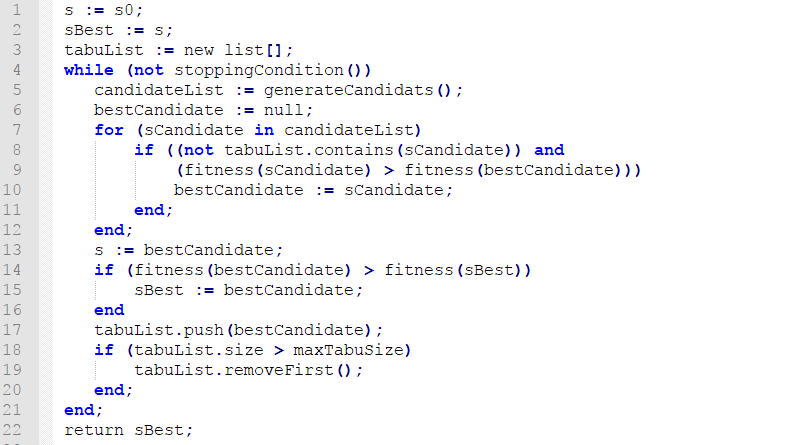
\includegraphics{PseudokodTabu}
	\caption{Pseudokod algorytmu Tabu search}
	\label{fig: AlgorytmTabu}
\end{figure}

\subsection{Sąsiedztwo rozwiązania}

Najważniejszym czynnikiem, od którego zależy sukces algorytmu jest poprawnie zdefiniowane sąsiedztwo, które będzie przeszukiwane w danej iteracji. Do sąsiedztwa powinny należeć rozwiązania różniące się w sposób nieznaczny od rozwiązania bieżącego. Jednak sąsiedztwo powinno umożliwiać algorytmowi przejście w każdy obszar przestrzeni rozwiązań. Sposób w jaki definiowane jest sąsiedztwo zależy od danego problemu i typu jego rozwiązań. Rozwiązania problemu mogą być reprezentowane np. przez wektory binarne, wektory liczb rzeczywistych, czy dowolne permutacje elementów zadanych zbiorów. Jeżeli na przykład rozwiązaniem będzie permutacja pewnego zbioru \textit{n} elementowego, to sąsiedztwem możemy określić jedno z trzech typów przejść (ruchów) między permutacjami:

\begin{itemize}
	\item wstaw(x, y) - wstawienie elementu y na pozycję x (permutacje z powtórzeniami),
	\item zamień(x, y) - zamiana elementów na pozycjach x i y,
	\item odwróć(x, y) - odwrócenie kolejności występowania elementów, począwszy od elementu o indeksie x, aż do elementu na pozycji y.
\end{itemize}

Sąsiedztwem danej permutacji będzie więc każda inna permutacja uzyskana za pomocą, wybranego na początku, sposobu modyfikacji bieżącej permutacji. Dzięki tak zdefiniowanemu sąsiedztwu możliwe jest łatwe zidentyfikowanie ruchu za pomocą pary indeksów (x, y). Para ta zostanie zapisana na liście tabu, a ruch ten będzie zablokowany przez następne iteracje.

Może się jednak okazać, że generowane sąsiedztwa są zbyt duże, by każdorazowo przeszukiwać je w całości. Stosowane jest wtedy zawężanie sąsiedztwa. Jednym ze sposobów zawężania jest losowy dobór sąsiedztwa. Wprowadza to element probabilistyczny do algorytmu, co zmniejsza prawdopodobieństwo powstania niepożądanych cykli. Jednak przy takim podejściu możemy pominąć obszary przestrzeni rozwiązań, w których znajduje się rozwiązanie optymalne.

\subsection{Kryteria aspiracji}

Może się zdarzyć, że zablokowanie pewnych ruchów doprowadzi do stagnacji procesu przeszukiwania lub całkowicie zablokuje kolejny ruch (np. w sytuacji, gdy wszystkie możliwe ruchy są na liście tabu). Jest to możliwe, ponieważ algorytm przechowuje tylko atrybuty rozwiązań, a nie całe rozwiązania. Kryterium aspiracji umożliwia zapobieganiu takiej sytuacji.
Spełnienie kryterium aspiracji pozwala na złamanie zakazu tabu, czyli wykonanie ruchu, który znajduje się na liście ostatnio wykonanych. Najpopularniejszym i najprostszym kryterium aspiracji jest uzyskanie najlepszego, nieznanego jak dotąd, wyniku. Musi być ono lepsze od aktualnie najlepszego w celu uniknięcia zapętleń. Jednak większość kryteriów aspiracji jest bardziej skomplikowana i opiera się na wyspecjalizowanym przewidywaniu możliwości powstania cyklu po wykonaniu określonego ruchu.

\subsection{Dywersyfikacji i intensyfikacja}

Ważnym aspektem algorytmu wyszukiwania z tabu jest pamięć długoterminowa. Służy ona do przechowywania danych o wykonanych już iteracjach i do budowania statystyk. Dzięki tym statystykom można modyfikować strategię poszukiwania. Głównym celem takich modyfikacji może być spełnienie jednego z dwóch kryteriów:
\begin{itemize}
	\item Intensyfikacja - jeżeli według statystyki, w danym obszarze znajduje się dużo dobrych rozwiązań to algorytm zagęści obszar poszukiwań. Dzięki temu istnieje szansa na znalezienie jeszcze lepszego rozwiązania w danym obszarze.
	\item Dywersyfikacja - jest to powiększenie obszaru poszukiwań. Najczęściej stosowanym sposobem jest nakładanie kary na ruchy, które powtarzają się w perspektywie dłuższego czasu. Efektem tego jest ,,przeniesienie" algorytmu w inne rejony poszukiwań, co zmniejsza szanse na pominięcie najlepszych rozwiązań.
\end{itemize}
Wykorzystanie intensyfikacji i dywersyfikacji w znaczniej mierze poprawia efektywność algorytmu, dlatego kryteria te są wykorzystywane w większości nowych wersji algorytmu \textit{Tabu Search}.







%   this is for BibTeX.  remove if you plan to write the references in the document
%\bibliographystyle{plplain}
\bibliographystyle{plain}
\bibliography{refs}

%adds the bibliography to the table of contents
\addcontentsline{toc}{chapter}
         {\protect\numberline{Bibliografia\hspace{-96pt}}}
         
%dodatki
\appendix
\chapter{Symbole przyjęte w pracy}
\label{app:symbole}

Jeśli w tekście nie wykazano inaczej, stosowane symbole należy rozumieć jako:

\begin{itemize}
\item[$f(x,y)$] - jasność piksela o współrzędnych $(x,y)$ w obrazie wejściowym,
\item[$g(x,y)$] - jasność piksela o współrzędnych $(x,y)$ w obrazie wynikowym,
\item[$t$, $t_i$] - wartości progowe,
\item[$G$] - liczba poziomów szarości obrazu; $G=256$,
\item[$P(i,j)$] - macierz GLCM,
\item[$M(i,j)$] - maska przetwarzania.
\end{itemize}


%%%%%%%%%%%%%%%%%%%%%%%%%%%%%%%%%%%%%%%%%%%%%%%%%%%%%%%%
\chapter{Inny, przykładowy dodatek}
\label{app:dodatekPrzyklad}

\end{document}